\textbf{Exercício}: Verificar o deslocamento horizontal (global e local) da estrutura abaixo em relação aos limites impostos pela NBR 6118 através do coeficiente $\gamma_z$, considerando somente a primeira combinação do ELU, sabendo-se que:

\begin{itemize}
	\item Edifício com térreo + 6 pavimentos;
	\item Altura entre pisos de 3 $m$;
	\item Carga acidental no andar-tipo de 191,52 $kN$;
	\item Carga acidental na cobertura de 63,84 $kN$;
	\item Carga permanente no andar-tipo de 1380,48 $kN$;
	\item Carga permanente na cobertura de 732,576 $kN$;
	\item Pilares de (12x40) $cm$;
	\item Quatro pilares na face do vento.
\end{itemize}

Nota: As unidades de carga descritas acima representam as reações de apoio das vigas nos pilares.

Dada a quantidade de valores para manuseio, recomenda-se para o leitor utilizar alguma planilha eletrônica para faciltar a compreensão. O primeiro passo é colocar as seguintes cargas no pórtico do presente exercício, atentando-se ao fato de que os valores de carga de vento ($H_v$) devem ser divididos pela quantidade de pilares na face do vento (4).

\begin{table}[H]
	\centering
	\caption{Valores de cota ($z$) e valores de carga de vento ($H_v$) para o presente exercício.}
	\begin{tabular}{c|c}
	\hline
	z ($m$) & $H_v$ ($kN$) \\ \hline
	3       & 19,255       \\
	6       & 22,740       \\
	9       & 25,065       \\
	12      & 26,857       \\
	15      & 28,333       \\
	18      & 29,602       \\
	21      & 15,358       \\ \hline
	\end{tabular}
\end{table}

Monta-se o pórtico no FTOOL e coloca-se 1/4 da carga de $H_v$ em cada pilar, de modo a ficar como segue:

\begin{figure}[H]
	\begin{center}
	\caption{Esquematização do exercício proposto e distribuição das cargas horizontais.}
    	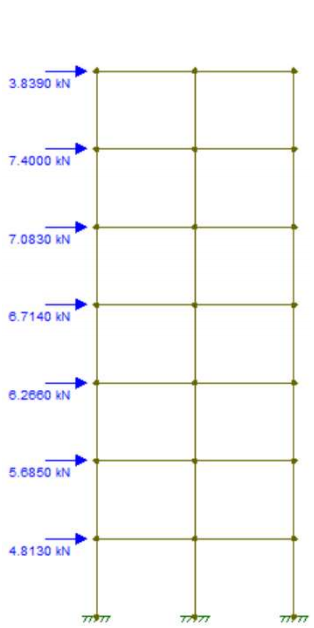
\includegraphics[width=0.4\textwidth]{Exercicios/Imagens/Exercicio-portico.png}
	\end{center}
\end{figure}

Neste exercício, o vento é considerado como efeito secundário, portanto, deve ser minorado por um coeficiente $\psi_0$, que no presente exercício equivale a 0,6 (valor para pressão dinâmica do vento para estruturas em geral, vide tabela 11.2 da NBR 6118).

Todo o exercício objetiva o encontro de $\gamma_z$ para verificar a estabilidade global do edifício e qual tipo de nó está presente na estrutura, com ele pode-se verificar se será necessário considerar os efeitos de 2ª ordem. Os parâmetros de $\gamma_z$ são $M_{1, total, d}$ e $\Delta M_{total, d}$, que são os momentos fletores causados pela carga horizontal final e a carga vertical, respectivamente.

O próximo passo é preencher a seguinte tabela:

\begin{table}[H]
\centering
\caption{Tabela a ser preenchida para facilitar o cálculo de $\gamma_z$.}
\label{tab:Tabela-exercicio-vento}
\begin{tabular}{c|c|c|ccc|c}
\hline
Andar & $F_d$ $minorada$ & $M_{1, total, d}$ & \multicolumn{1}{c|}{$P_d$} & \multicolumn{1}{c|}{$d_{horiz}$} & $d_{horiz}$ $minorada$ & $\Delta M_{total, d}$ \\
 & ($kN$) & ($kN\cdot cm$) & \multicolumn{1}{c|}{($kN$)} & \multicolumn{1}{c|}{($cm$) (FTOOL)} & ($cm$) & ($kN\cdot cm$) \\ \hline
1 &  &  & \multicolumn{1}{c|}{} & \multicolumn{1}{c|}{} &  &  \\
2 &  &  & \multicolumn{1}{c|}{} & \multicolumn{1}{c|}{} &  &  \\
3 &  &  & \multicolumn{1}{c|}{} & \multicolumn{1}{c|}{} &  &  \\
4 &  &  & \multicolumn{1}{c|}{} & \multicolumn{1}{c|}{} &  &  \\
5 &  &  & \multicolumn{1}{c|}{} & \multicolumn{1}{c|}{} &  &  \\
6 &  &  & \multicolumn{1}{c|}{} & \multicolumn{1}{c|}{} &  &  \\
7 &  &  & \multicolumn{1}{c|}{} & \multicolumn{1}{c|}{} &  &  \\ \hline
Total &  &  &  &  &  &  \\ \cline{1-1} \cline{3-3} \cline{7-7} 
\end{tabular}
\end{table}

Onde $F_{d, minorada}$ é a carga de vento minorada (já que o respectivo efeito é considerado secundário; é a minoração de $H_v$), $M_{1, total, d}$ é o momento fletor que a carga horizontal causa na estrutura, $Pd$ é a carga vertical atuante na estrutura ($g+q$) unitária de cada andar, $d_{horiz}$ é o deslocamento horizontal causado pela carga horizontal (obtido no FTOOL), $d_{horiz}\;minorada$ é o deslocamento horizontal causado pela carga horizontal minorada (novamente, o efeito dos ventos está sendo considerado como secundário no exercício) e $\Delta M_{total, d}$ é o momento fletor gerado pelo deslocamento horizontal causado pelas cargas verticais. O 7º pavimento é a cobertura.

Calcula-se $F_{d, minorada}$ pela equação:
\begin{equation}F_{d, minorada}=1,4\cdot\psi_0\cdot H_v\end{equation}

Por exemplo, para o 1º e 2º andar, respectivamente: $$F_{d, minorada}=1,4\cdot 0,6\cdot 19,255\;kN=16,1742\;kN$$, $$F_{d, minorada}=1,4\cdot 0,6\cdot 22,740\;kN=19,1016\;kN$$

Preenchendo a respectiva coluna na Tabela~\ref{tab:Tabela-exercicio-vento}, tem-se:

\begin{table}[H]
\centering
\begin{tabular}{c|c|c|ccc|c}
\hline
Andar & $F_d$ $minorado$ & $M_{1, total, d}$ & \multicolumn{1}{c|}{$P_d$} & \multicolumn{1}{c|}{$d_{horiz}$} & $d_{horiz}$ $minorada$ & $\Delta M_{total, d}$ \\
 & ($kN$) & ($kN\cdot cm$) & \multicolumn{1}{c|}{($kN$)} & \multicolumn{1}{c|}{($cm$) (FTOOL)} & ($cm$) & ($kN\cdot cm$) \\ \hline
1 & 16,1742 &  & \multicolumn{1}{c|}{} & \multicolumn{1}{c|}{} &  &  \\
2 & 19,1016 &  & \multicolumn{1}{c|}{} & \multicolumn{1}{c|}{} &  &  \\
3 & 21,0546 &  & \multicolumn{1}{c|}{} & \multicolumn{1}{c|}{} &  &  \\
4 & 22,5599 &  & \multicolumn{1}{c|}{} & \multicolumn{1}{c|}{} &  &  \\
5 & 23,7997 &  & \multicolumn{1}{c|}{} & \multicolumn{1}{c|}{} &  &  \\
6 & 24,8657 &  & \multicolumn{1}{c|}{} & \multicolumn{1}{c|}{} &  &  \\
7 & 12,9007 &  & \multicolumn{1}{c|}{} & \multicolumn{1}{c|}{} &  &  \\ \hline
Total &  &  &  &  &  &  \\ \cline{1-1} \cline{3-3} \cline{7-7} 
\end{tabular}
\end{table}

Agora, pode-se calcular o momento fletor ($M_{1, total, d}$) causado por cada força horizontal ($F_{d, minorada}$) em relação à base do edifício. Para o 1º e 2º andar, tem-se, respectivamente:
$$M_{1, total, d}=F_{d, minorada}\cdot z=16,1742\;kN\cdot 300\;cm=4852,26\;kN\cdot cm$$
$$M_{1, total, d}=F_{d, minorada}\cdot z=19,1016\;kN\cdot 600\;cm=11460,96\;kN\cdot cm$$

Note que a cota ($z$) é a altura que o respectivo pavimento está da base. Preenchendo a respectiva coluna na Tabela~\ref{tab:Tabela-exercicio-vento}, tem-se:

\begin{table}[H]
\centering
\begin{tabular}{c|c|c|ccc|c}
\hline
Andar & $F_d$ $minorada$ & $M_{1, total, d}$ & \multicolumn{1}{c|}{$P_d$} & \multicolumn{1}{c|}{$d_{horiz}$} & $d_{horiz}$ $minorada$ & $\Delta M_{total, d}$ \\
 & ($kN$) & ($kN\cdot cm$) & \multicolumn{1}{c|}{($kN$)} & \multicolumn{1}{c|}{($cm$) (FTOOL)} & ($cm$) & ($kN\cdot cm$) \\ \hline
1 & 16,1742 & 4852,26 & \multicolumn{1}{c|}{} & \multicolumn{1}{c|}{} &  &  \\
2 & 19,1016 & 11460,96 & \multicolumn{1}{c|}{} & \multicolumn{1}{c|}{} &  &  \\
3 & 21,0546 & 18949,14 & \multicolumn{1}{c|}{} & \multicolumn{1}{c|}{} &  &  \\
4 & 22,5599 & 27071,88 & \multicolumn{1}{c|}{} & \multicolumn{1}{c|}{} &  &  \\
5 & 23,7997 & 35699,55 & \multicolumn{1}{c|}{} & \multicolumn{1}{c|}{} &  &  \\
6 & 24,8657 & 44758,26 & \multicolumn{1}{c|}{} & \multicolumn{1}{c|}{} &  &  \\
7 & 12,9007 & 27091,47 & \multicolumn{1}{c|}{} & \multicolumn{1}{c|}{} &  &  \\ \hline
Total &  & 169883,53 &  &  &  &  \\ \cline{1-1} \cline{3-3} \cline{7-7} 
\end{tabular}
\end{table}

A carga vertical $P_d$ é a mesma para todos os pavimentos tipo, sendo: $$P_d=g+q=1,4\cdot1380,48\;kN+1,4\cdot191,52\;kN=2200,8\;kN$$

A carga vertical $P_d$ para a cobertura é: $$P_d=g+q=1,4\cdot 732,576\;kN+1,4\cdot63,84\;kN=1114,9824\;kN$$

Preenchendo a respectiva coluna na Tabela~\ref{tab:Tabela-exercicio-vento}, tem-se:

\begin{table}[H]
\centering
\begin{tabular}{c|c|c|ccc|c}
\hline
Andar & $F_d$ $minorada$ & $M_{1, total, d}$ & \multicolumn{1}{c|}{$P_d$} & \multicolumn{1}{c|}{$d_{horiz}$} & $d_{horiz}$ $minorada$ & $\Delta M_{total, d}$ \\
 & ($kN$) & ($kN\cdot cm$) & \multicolumn{1}{c|}{($kN$)} & \multicolumn{1}{c|}{($cm$) (FTOOL)} & ($cm$) & ($kN\cdot cm$) \\ \hline
1 & 16,1742 & 4852,26 & \multicolumn{1}{c|}{2200,800} & \multicolumn{1}{c|}{} &  &  \\
2 & 19,1016 & 11460,96 & \multicolumn{1}{c|}{2200,800} & \multicolumn{1}{c|}{} &  &  \\
3 & 21,0546 & 18949,14 & \multicolumn{1}{c|}{2200,800} & \multicolumn{1}{c|}{} &  &  \\
4 & 22,5599 & 27071,88 & \multicolumn{1}{c|}{2200,800} & \multicolumn{1}{c|}{} &  &  \\
5 & 23,7997 & 35699,55 & \multicolumn{1}{c|}{2200,800} & \multicolumn{1}{c|}{} &  &  \\
6 & 24,8657 & 44758,26 & \multicolumn{1}{c|}{2200,800} & \multicolumn{1}{c|}{} &  &  \\
7 & 12,9007 & 27091,47 & \multicolumn{1}{c|}{1114,9824} & \multicolumn{1}{c|}{} &  &  \\ \hline
Total &  & 169883,53 &  &  &  &  \\ \cline{1-1} \cline{3-3} \cline{7-7} 
\end{tabular}
\end{table}

O valor de $d_{horiz}$ é obtido através do software livre FTOOL. Preenchendo a respectiva coluna na Tabela~\ref{tab:Tabela-exercicio-vento}, tem-se:

\begin{table}[H]
\centering
\begin{tabular}{c|c|c|ccc|c}
\hline
Andar & $F_d$ $minorada$ & $M_{1, total, d}$ & \multicolumn{1}{c|}{$P_d$} & \multicolumn{1}{c|}{$d_{horiz}$} & $d_{horiz}$ $minorada$ & $\Delta M_{total, d}$ \\
 & ($kN$) & ($kN\cdot cm$) & \multicolumn{1}{c|}{($kN$)} & \multicolumn{1}{c|}{($cm$) (FTOOL)} & ($cm$) & ($kN\cdot cm$) \\ \hline
1 & 16,1742 & 4852,26 & \multicolumn{1}{c|}{2200,800} & \multicolumn{1}{c|}{0,3228} &  &  \\
2 & 19,1016 & 11460,96 & \multicolumn{1}{c|}{2200,800} & \multicolumn{1}{c|}{0,7735} &  &  \\
3 & 21,0546 & 18949,14 & \multicolumn{1}{c|}{2200,800} & \multicolumn{1}{c|}{1,1816} &  &  \\
4 & 22,5599 & 27071,88 & \multicolumn{1}{c|}{2200,800} & \multicolumn{1}{c|}{1,5184} &  &  \\
5 & 23,7997 & 35699,55 & \multicolumn{1}{c|}{2200,800} & \multicolumn{1}{c|}{1,7743} &  &  \\
6 & 24,8657 & 44758,26 & \multicolumn{1}{c|}{2200,800} & \multicolumn{1}{c|}{1,9440} &  &  \\
7 & 12,9007 & 27091,47 & \multicolumn{1}{c|}{1114,9824} & \multicolumn{1}{c|}{2,0326} &  &  \\ \hline
Total &  & 169883,53 &  &  &  &  \\ \cline{1-1} \cline{3-3} \cline{7-7} 
\end{tabular}
\end{table}

O valor contido na tabela de $d_{horiz}$ foi obtido no FTOOL a partir da carga $H_v$ (não minorada). Para obtermos $d_{horiz, minorada}$, deve-se minorar $d_{horiz}$ pelos mesmos fatores utilizados para minorar $H_v$. Para o 1º e 2º andar, tem-se:
$$d_{horiz, minorada}=1,4\cdot\psi_0\cdot d_{horiz}=1,4\cdot0,6\cdot 0,3228\;cm=0,2712\;cm$$ $$d_{horiz, minorada}=1,4\cdot\psi_0\cdot d_{horiz}=1,4\cdot0,6\cdot 0,7735\;cm=0,6497\;cm$$

Preenchendo a respectiva coluna na Tabela~\ref{tab:Tabela-exercicio-vento}, tem-se:

\begin{table}[H]
\centering
\begin{tabular}{c|c|c|ccc|c}
\hline
Andar & $F_d$ $minorada$ & $M_{1, total, d}$ & \multicolumn{1}{c|}{$P_d$} & \multicolumn{1}{c|}{$d_{horiz}$} & $d_{horiz}$ $minorada$ & $\Delta M_{total, d}$ \\
 & ($kN$) & ($kN\cdot cm$) & \multicolumn{1}{c|}{($kN$)} & \multicolumn{1}{c|}{($cm$) (FTOOL)} & ($cm$) & ($kN\cdot cm$) \\ \hline
1 & 16,1742 & 4852,26 & \multicolumn{1}{c|}{2200,800} & \multicolumn{1}{c|}{0,3228} & 0,2712 &  \\
2 & 19,1016 & 11460,96 & \multicolumn{1}{c|}{2200,800} & \multicolumn{1}{c|}{0,7735} & 0,6497 &  \\
3 & 21,0546 & 18949,14 & \multicolumn{1}{c|}{2200,800} & \multicolumn{1}{c|}{1,1816} & 0,9925 &  \\
4 & 22,5599 & 27071,88 & \multicolumn{1}{c|}{2200,800} & \multicolumn{1}{c|}{1,5184} & 1,2755 &  \\
5 & 23,7997 & 35699,55 & \multicolumn{1}{c|}{2200,800} & \multicolumn{1}{c|}{1,7743} & 1,4904 &  \\
6 & 24,8657 & 44758,26 & \multicolumn{1}{c|}{2200,800} & \multicolumn{1}{c|}{1,9440} & 1,6330 &  \\
7 & 12,9007 & 27091,47 & \multicolumn{1}{c|}{1114,9824} & \multicolumn{1}{c|}{2,0326} & 1,7074 &  \\ \hline
Total &  & 169883,53 &  &  &  &  \\ \cline{1-1} \cline{3-3} \cline{7-7} 
\end{tabular}
\end{table}

A última coluna da tabela, $\Delta M_{total, d}$, que é o momento fletor causado pela carga vertical vezes a excentricidade causada pela carga horizontal, é, para o 1º e 2º andar, respectivamente:
$$\Delta M_{total, d}=P_d\cdot d_{horiz, minorada}=2200,800\;kN\cdot0,2712\;cm=596,7513\;kN\cdot cm$$
$$\Delta M_{total, d}=P_d\cdot d_{horiz, minorada}=2200,800\;kN\cdot0,6497\;cm=1429,9478\;kN\cdot cm$$

Preenchendo a respectiva coluna na Tabela~\ref{tab:Tabela-exercicio-vento}, tem-se:

\begin{table}[H]
\centering
\begin{tabular}{c|c|c|ccc|c}
\hline
 & $F_d$ $minorada$ & $M_{1, total, d}$ & \multicolumn{1}{c|}{$P_d$} & \multicolumn{1}{c|}{$d_{horiz}$} & $d_{horiz}$ $minorada$ & $\Delta M_{total, d}$ \\
 & ($kN$) & ($kN\cdot cm$) & \multicolumn{1}{c|}{($kN$)} & \multicolumn{1}{c|}{($cm$) (FTOOL)} & ($cm$) & ($kN\cdot cm$) \\ \hline
1 & 16,1742 & 4852,26 & \multicolumn{1}{c|}{2200,800} & \multicolumn{1}{c|}{0,3228} & 0,2712 & 596,7513 \\
2 & 19,1016 & 11460,96 & \multicolumn{1}{c|}{2200,800} & \multicolumn{1}{c|}{0,7735} & 0,6497 & 1429,9478 \\
3 & 21,0546 & 18949,14 & \multicolumn{1}{c|}{2200,800} & \multicolumn{1}{c|}{1,1816} & 0,9925 & 2184,3908 \\
4 & 22,5599 & 27071,88 & \multicolumn{1}{c|}{2200,800} & \multicolumn{1}{c|}{1,5184} & 1,2755 & 2807,0236 \\
5 & 23,7997 & 35699,55 & \multicolumn{1}{c|}{2200,800} & \multicolumn{1}{c|}{1,7743} & 1,4904 & 3280,0987 \\
6 & 24,8657 & 44758,26 & \multicolumn{1}{c|}{2200,800} & \multicolumn{1}{c|}{1,9440} & 1,6330 & 3593,8184 \\
7 & 12,9007 & 27091,47 & \multicolumn{1}{c|}{1114,9824} & \multicolumn{1}{c|}{2,0326} & 1,7074 & 1903,6990 \\ \hline
Total &  & 169883,53 &  &  &  & 15795,7296 \\ \cline{1-1} \cline{3-3} \cline{7-7} 
\end{tabular}
\end{table}

Agora, pode-se calcular o valor de $\gamma_z$ para verificarmos o tipo de nó presente na estrutura.
$$\gamma_z=\frac{1}{1-\frac{\Delta M_{total, d}}{M_{1, total, d}}}=\frac{1}{1-\frac{15795,7296\;kN}{169883,53\;kN}}\approx1,1025$$

Portanto, o tipo de nó é móvel ($1,1<\gamma_z\leqslant1,3$). Nós móveis obriga a definição dos efeitos de 2ª ordem para as cargas horizontais. Para isso, a NBR 6118 permite majorar a carga de vento com a equação:
\begin{equation}H_{v2}=H_v\cdot0,95\cdot\gamma_z\end{equation}

Onde $H_{v2}$ é a nova carga de vento majorada em $kN$, $H_v$ é a carga de vento nos nós da estrutura em $kN$ e $\gamma_z$ é o coeficiente de estabilidade global (adimensional).

Essa nova carga horizontal ($H_{v2}/4$) deve ser colocada no lugar da antiga ($H_v/4$) no FTOOL objetivando encontrar novos deslocamentos horizontais. Pode-se, então, montar a seguinte tabela para facilitar os cálculos:

\begin{table}[H]
\centering
\caption{Tabela a ser preenchida para verificação de deslocamento horizontal em nós móveis.}
\label{tab:Tabela-exercicio-deslocamento-nos-moveis}
\begin{tabular}{c|c|c|c|c|c}
\hline
\begin{tabular}[c]{@{}c@{}}z\\ ($m$)\end{tabular} & \begin{tabular}[c]{@{}c@{}}$H_{v2}$\\ ($kN$)\end{tabular} & \begin{tabular}[c]{@{}c@{}}$\frac{H_{v2}}{4}$\\ ($kN$)\end{tabular} & \begin{tabular}[c]{@{}c@{}}$d_{horiz, 2}$\\ FTOOL ($cm$)\end{tabular} & \begin{tabular}[c]{@{}c@{}}$d_{horiz, 2}\cdot\psi_1$\\ ($cm$)\end{tabular} & \begin{tabular}[c]{@{}c@{}}$\Delta_{desloc, 2}$\\ ($cm$)\end{tabular} \\ \hline
3                                                 & 20,1674                                                                      & 5,0419                                                              & 0,3448                                                                &                                                                            &                                                                    \\
6                                                 & 23,8176                                                                      & 5,9544                                                              & 0,8263                                                                &                                                                            &                                                                    \\
9                                                 & 26,2527                                                                      & 6,5632                                                              & 1,2622                                                                &                                                                            &                                                                    \\
12                                                & 28,1296                                                                      & 7,0324                                                              & 1,6221                                                                &                                                                            &                                                                    \\
15                                                & 29,6756                                                                      & 7,4189                                                              & 1,8954                                                                &                                                                            &                                                                    \\
18                                                & 31,0047                                                                      & 7,7512                                                              & 2,0767                                                                &                                                                            &                                                                    \\
21                                                & 16,0857                                                                      & 4,0214                                                              & 2,1713                                                                &                                                                            &                                                                    \\ \hline
\end{tabular}
\end{table}

O coeficiente $\psi_1$ na penúltima coluna é o valor de pressão dinâmica do vento nas estruturas em geral (0,3). O valor do produto ($d_{horiz, 2}\cdot\psi_1$) diz respeito ao \textbf{deslocamento global} da estrutura. O valor de $\Delta_{desloc, 2}$ diz respeito a variação de deslocamento entre um pavimento e o logo abaixo, ou seja, o \textbf{deslocamento local}. O referido produto para o 6º pavimento e cobertura são, respectivamente:
$$d_{horiz}\cdot\psi_1=2,0767\cdot0,3=0,6230\;cm$$
$$d_{horiz}\cdot\psi_1=2,1713\cdot0,3=0,6513\;cm$$

O valor de deslocamento local de cada pavimento deve ser obtido da seguinte forma:
\begin{equation}{\Delta_{desloc, 2}}_i={(d_{horiz}\cdot\psi_1)}_i-{(d_{horiz}\cdot\psi_1)}_{i-1}\end{equation}

O valor de $\Delta_{desloc, 2}$ para a cobertura é, portanto: $$\Delta_{desloc, 2}=0,6513-0,6230=0,0283\;cm$$

Completanto a Tabela~\ref{tab:Tabela-exercicio-deslocamento-nos-moveis}, tem-se:

\begin{table}[H]
\centering
\begin{tabular}{c|c|c|c|c|c}
\hline
\begin{tabular}[c]{@{}c@{}}z\\ ($m$)\end{tabular} & \begin{tabular}[c]{@{}c@{}}$H_v\cdot0,95\cdot\gamma_z$\\ ($kN$)\end{tabular} & \begin{tabular}[c]{@{}c@{}}$\frac{H_{v2}}{4}$\\ ($kN$)\end{tabular} & \begin{tabular}[c]{@{}c@{}}$d_{horiz, 2}$\\ FTOOL ($cm$)\end{tabular} & \begin{tabular}[c]{@{}c@{}}$d_{horiz, 2}\cdot\phi_1$\\ ($cm$)\end{tabular} & \begin{tabular}[c]{@{}c@{}}$\Delta desloc 2$\\ ($cm$)\end{tabular} \\ \hline
3                                                 & 20,1674                                                                      & 5,0419                                                              & 0,3448                                                                & 0,10344                                                                    & 0,1034                                                             \\
6                                                 & 23,8176                                                                      & 5,9544                                                              & 0,8263                                                                & 0,24789                                                                    & 0,1445                                                             \\
9                                                 & 26,2527                                                                      & 6,5632                                                              & 1,2622                                                                & 0,37866                                                                    & 0,1308                                                             \\
12                                                & 28,1296                                                                      & 7,0324                                                              & 1,6221                                                                & 0,48663                                                                    & 0,1080                                                             \\
15                                                & 29,6756                                                                      & 7,4189                                                              & 1,8954                                                                & 0,56862                                                                    & 0,0820                                                             \\
18                                                & 31,0047                                                                      & 7,7512                                                              & 2,0767                                                                & 0,62301                                                                    & 0,0544                                                             \\
21                                                & 16,0857                                                                      & 4,0214                                                              & 2,1713                                                                & 0,65139                                                                    & 0,0283                                                             \\ \hline
\end{tabular}
\end{table}

Nota: Alguns valores podem ficar bem próximos, já que foram feitos em planilha eletrônica. O importante é entender o processo lógico por trás do método.

Por fim, verifica-se se os deslocamentos estão dentro do aceitável pela NBR 6118, que são:

\begin{itemize}
	\item Para o topo: $H/1700$, onde $H$ é a cota da cobertura (verificação global);
	\item Para entre pisos: $H_{pisos}/850$, onde $H_{pisos}$ é a altura piso a piso (verificação local).
\end{itemize}

Para o topo, tem-se: $$H/1700=2100\;cm/1700\approx1,2553\;cm>0,6513\;cm\;(OK)$$
Para o entre pisos, checa-se com o maior valor de $\Delta_{desloc, 2}$ presente na Tabela~\ref{tab:Tabela-exercicio-deslocamento-nos-moveis}. Tem-se: $$H_{pisos}/850=300\;cm/850\approx0,3529\;cm>0,1445\;cm\;(OK)$$

Os deslocamentos global e local atendem às exigencias da NBR 6118.